\chapter{Wstęp}
W ostatnich latach zarysowuje się coraz większa potrzeba wdrażania systemów informatycznych. Ta tendencja związana  jest przede wszystkim z usprawnianiem procesów biznesowych, ze wzrostem wydajności pracy, identyfikacją oraz minimalizacją błędów lub nieefektywnych działań w firmach. Występuje wiele ich rodzajów: CRM (ang. \emph{Customer Relationship Managment}) - wspomagające zarządzanie relacjami z klientami, ERP (ang. \emph{Enterprise Resource Planning}) – wspomagające zarządzanie i planowanie zasobami firmy czy też BPM (ang. \emph{Business Process Managment}) – wspomagające zarządzanie procesami biznesowymi. 

Wprowadzanie systemów informatycznych do organizacji może wywoływać różnorodne efekty: techniczne (związane z zastosowaniem techniki komputerowej - zwiększenie szybkości i dokładności przetwarzania, wzrost szczegółowości oraz poprawa bezpieczeństwa dla informacji), ekonomiczne (związane pośrednio ze wzrostem efektywności i szybkości podejmowania decyzji), organizacyjne (przede wszystkim związane są z usprawnieniami struktury organizacyjnej i procesów zachodzących w przedsiębiorstwie - podniesienie sprawności obiegu dokumentów, eliminacja zbędnej pracy administracyjnej, poprawa koordynacji zadań oraz eliminacja błędów), socjopsychologiczne (związane z rozszerzeniem zakresu komunikacji pomiędzy pracownikami, usprawnieniem systemu ocen pracowniczych oraz polepszeniem kultury organizacyjnej). \cite{EfektyZasSys}

Utworzenie systemu informatycznego dla dużych firm i instytucji nie stanowi zadania trywialnego. Banki, uczelnie lub urzędy charakteryzują się często stosunkowo złożoną strukturą organizacyjną oraz panują w nich skomplikowane procesy wewnętrzne. Powstaje wówczas problem z formalnym opisem danej jednostki – niezbędnym do utworzenia funkcjonalnego, spełniającego wymagania klienckie systemu informatycznego. Bardzo istotnym elementem jest wówczas stosowanie odpowiedniej metodyki, która pozwoli na usystematyzowane podejście do projektowania tego rodzaju systemów. 

\section{Cel pracy}
Podstawowym celem pracy jest utworzenie metodyki projektowania architektury korporacyjnej opierającej się na wykorzystaniu języka SoaML. Dotychczas utworzono już podobne metodyki, jednakże żadna nie była w stanie w pełni sprostać wszystkim wymaganiom stawianym przez problematykę architektury korporacyjnej.

Projekt metodyki powstanie w oparciu o wybranie najmocniejszych stron oraz pominięciu wad istniejących metodyk. Podjęta zostanie również próba wdrożenia innowacyjnych elementów, które będą miały na celu usprawnienie procesu projektowania architektury korporacyjnej.

Zaprojektowana metodyka zostanie również poddana weryfikacji i testom przy tworzeniu niewielkiego systemu bankowego.

\section{Pozostałe założenia dla pracy}
Oprócz założenia głównego dla pracy (utworzenie metodyki projektowania architektury korporacyjnej) postawiono kilka innych, które powinna realizować:
\begin{itemize}
\item{zdefiniowanie architektury korporacyjnej oraz wyjaśnienie terminów z nią powiązanych,}
\item{omówienie obecnych metodyk wykorzystywanych do projektowania architektury korporacyjnej,}
\item{omówienie języków wykorzystywanych do projektowania architektury korporacyjnej,}
\item{weryfikacja koncepcji autorskiej metody przy wdrożeniu przykładowego systemu bankowego.}
\end{itemize}

\chapter{Charakterystyka architektury korporacyjnej}

\section{Wstęp}
Żyjemy w coraz szybciej zmieniającym się świecie. Stan ten powoduje, że współczesne organizacje muszą charakteryzować się coraz większą elastycznością. Jednocześnie ich poziom złożoności, jak również skala działania znacznie rosną.\cite{SobArchKorpDobrPr}

Do innych problemów zalicza się również niejednorodność procesów biznesowych w poszczególnych jednostkach. Może wywoływać to trudności w stosowaniu wspólnych procedur postępowania w ramach całego przedsiębiorstwa. Rozwój i utrzymywanie zbyt wielu platform, gdy systemy tworzone były w różnych technologiach może prowadzić również do trudności we współdziałaniu tychże systemów.

W rozdziale zostanie zdefiniowany termin \quotedblbase architektura korporacyjna\textquotedblright oraz wyjaśnione najważniejsze elementy z nim związane. Podjęta będzie również tematyka \quotedblbase architektury zorientowanej na usługi\textquotedblright oraz to jak ją zaadaptować do architektury korporacyjnej. 

\section{Definicje głównych pojęć związanych z architekturą korporacyjną}
Projektując architekturę korporacyjną (ang. \textit{Enterprise Architecture} należy dobrze rozumieć terminy z nią powiązane. W sekcji tej zostanie dokonany przegląd głównych pojęć odnoszących się do architektury korporacyjnej oraz podjęta próba ich zdefiniowania.

Słowo \quotedblbase architektura\textquotedblright w ujęciu do oprogramowania stanowi zbiór podstawowych decyzji związanych z oprogramowaniem lub rozwiązaniem programistycznym - zaprojektowanym z reguły tak, aby sprostać wszelkim atrybutom jakościowym (wymaganiom architektonicznym) danego projektu. Architektura tego typu zawiera z reguły główne komponenty, atrybuty oraz współdziałania (zachowanie i interakcje) umożliwiające spełnianie atrybutów jakościowych. Architektura może być wyrażona na więcej niż jednym poziomie abstrakcji, gdzie liczba poziomów zależy od rozmiaru i złożoności projektu. Termin ten posiada również powszechnie akceptowany opis w standardzie IEEE, który określa ją jako \quotedblbase podstawowe koncepcje lub właściwości systemu w jego  środowisku zawarte w jego elementach, relacjach oraz zasadach projektowania i rozwoju\textquotedblright (IEEE 42010). \cite{SOAWzorceArch}

Twórcy standardu uzupełniają tą definicję o następujące komentarze: 
\begin{itemize}
\item{Nazwa \quotedblbase architektura\textquotedblright nawiązuje do zestawu podstawowych (a nie wszystkich) właściwości systemu (rozpatrywanego jako całość), które określają jego formę i funkcje oraz związane z nim wartości, koszt i ryzyko.}
\item{Architektura systemu odróżniana jest od jego opisu i nie musi być udokumentowana. Opis architektury stanowi próbę wyrażenia pewnej koncepcji systemu, tak aby móc podzielić się nią z innymi. Architektura jest pewnym abstraktem, natomiast opis jest próbą uchwycenia tego abstraktu.
W definicji wprowadzono również dwa rozłączne podejścia do architektury - rozumienie jej jako pewnej koncepcji systemu, która istnieje w ludzkim  umyśle oraz jako percepcji właściwości systemu.}
\item{Architektura opisywana jest zawsze w pewnym kontekście. Zrozumienie podstawowych właściwości systemu systemu, wiąże się z odniesieniem do jego otoczenia, środowiska i interesariuszy.}
\end{itemize}

Kolejnym kluczowym terminem jest \quotedblbase korporacja\textquotedblright (ang. \textit{enterprise}. Pojęcie korporacja rozpatrywane jest najczęściej w kontekście całej jednostki organizacyjnej. Przyjmowane są różne jego różne definicje:
\begin{itemize}
\item{Zbiór aktywności w określonej dziedzinie z aktorami, których łączy wspólny cel.}
\item{Zorganizowany zbiór zasobów, które uczestniczą w wykonywaniu określonych procesów.}
\item{System istniejący w celu realizacji jednej lub wielu misji w określonym środowsiku.}
\item{Zbiór organizacji posiadających wspólny zbiór celów lub wspólne raportowanie finansowe.}
\end{itemize}

Wyraz korporacja wywodzi się z łacińskiego słowa \quotedblbase corporation\textquotedblright oznaczającego związek, połączenie części. Nie istnieje obowiązująca definicja dla tego terminu, jako organizacji gospodarczej. 

Według jednej z definicji jest to duża organizacja, zarządzana przez grupę specjalistów (kadrę zarządzającą), silnie oddziałująca na otoczenie zewnętrzne, posiadająca wyrazistą kulturę organizacyjną. Ma złożoną strukturę wewnętrzną, działającą na podstawie strategii długookresowych.

W przypadku organizacji gospodarczych za korporacją może być uznawane przedsiębiorstwo lub jego część (np. zakład). W przypadku jednostek administracji rządowej korporację może stanowić cała administracja rządowa (wszystkie jej jednostki), resort lub jego fragment.

Współcześnie uważa się, że korporacją - w rozumieniu architektury korporacyjnej - może być również tak zwane rozszerzone przedsiębiorstwo (\quotedblbase extended enterprise\textquotedblright). Ta kategoria przedsiębiorstwa definiowana jest jako zbiór jednostek prawnych, które są związane zintegrowanym łańcuchem wartości dodanej, dzięki czemu następuje zwiększenie wartości dostarczonej dla klientów.\cite{SobArchKorpDobrPr} 

\section{Wprowadzenie do architektury korporacyjnej}
Architektura korporacyjna (ang. \emph{enterprise architecture}) jest spojrzeniem na całość organizacji. Stanowi opis struktury i funkcji komponentów takich jak: zasoby danych, strategia, procesy biznesowe, jednostki organizacyjne, systemy informatyczne oraz infrastruktura teleinformatyczna. Opisuje stan obecny i docelowy oraz proces przejścia między tymi stanami w organizacji.\cite{ArchKorpSob}

Mimo, że architektura korporacyjna jest kojarzona głównie z technologią informatyczną, to przede wszystkim nawiązuje do metod optymalizacji procesów, wskazując architekturę biznesową, metody zarządzania efektywnością oraz organizacyjne uporządkowanie procesów\cite{ArchKorpSzymSup}

Architekturze korporacyjnej przypisuje się kilka znaczeń: atrybutowe, rzeczowe oraz czynnościowe.

W ujęciu atrybutowym uważana jest za zbiór właściwości danej organizacji (oraz relacji między nimi) koniecznych do zapewnienia realizacji jej celów. Architektura korporacyjna stanowi nieodłączną właściwość każdej organizacji. Jej jakość może być rozpatrywana w odniesieniu do efektywności realizacji istniejących celów strategicznych analizowanej organizacji.\cite{ArchKorpSob}

W ujęciu rzeczowym architektura korporacyjna definiowana jest jako formalna reprezentacja właściwości danej organizacji. W znaczeniu tym rozpatruje się ją również jako misję całej organizacji - informacje i zasoby techniczne niezbędne do realizacji zakładanych celów oraz proces przejścia związany z wdrażaniem nowych rozwiązań technicznych w nawiązaniu do zmian strategicznych w organizacji.\cite{ArchKorpSob}

Spojrzenie czynnościowe zakłada definicję architektury korporacyjnej jako zadań i umiejętności zarządzania tym, co jest opisane w definicji atrybutowej.\cite{ArchKorpSzymSup}

Podejście prezentowane w \emph{A Practical Guide to Federal Enterprise Architecture} uwzględnia aspekt transformacji organizacji w obszarze objętym architekturą korporacyjną, który jest immanentną cechą złożonych systemów adaptacyjnych.\cite{ArchKorpSob} 

A. Goikoetxea definiuje architekturę korporacyjną (EA) jako ośmioelemntową strukturę, składającą się z następujących zbiorów:

\begin{center}
\begin{equation}EA: \{R, B, A, D, S, T, C, M\},\end{equation}
\end{center}

gdzie:
\begin{itemize}
\item{$R = (r_{1}, r_{2},..., r_{n})$ - zbiór zawierający wszystkie wymagania systemowe - funkcjonalne i niefunkcjonalne, procesy, działania oraz reguły biznesowe.}
\item{$B = (b_{1}, b_{2},..., b_{p})$ - zbiór procesów biznesowych realizowanych w ramach organizacji. Metadane na temat wejść i wyjść dla każdego procesu zawarte są w zbiorze $C$.}
\item{$A = (a_{1}, a_{2},..., a_{q})$ - zbiór aplikacji biznesowych, funkcjonujących w ramach organizacji, które udostępniają usługi służące do implementacji procesów biznesowych. Metadane na temat relacji między tymi systemami przechowywane są w zbiorze $C$.}
\item{$D = (d_{1}, d_{2},..., d_{g})$ - zbiór danych, które konstytuują zasoby informacyjne organizacji. Metadane na temat organizacji tych danych, więzów integralności, reguł zarządzania przechowywane są w zbiorze $C$.}
\item{$S = (s_{1}, s_{2},..., s_{k})$ - zbiór systemów oprogramowania funkcjonujących w ramach organizacji umożliwiających realizację usług biznesowych przez aplikacje biznesowe. Metadane na temat wejść i wyjść poszczególnych aplikacji, interfejsy oraz standardy wytwarzania tych systemów przechowywane są w zbiorze $C$.}
\item{$T - (t_{1}, t_{2},..., t_{w})$ - zbiór komponentów technicznych organizacji - zarówno programowych (na przykład systemy operacyjne), jak i sprzętowych - niezbędnych do funkcjonowania systemów oprogramowania ze zbioru $A$.}
\item{$C = (c_{1}, c_{2},..., c_{h})$ - zbiór ograniczeń, które występują podczas tworzenia architektury korporacyjnej (takich jak np. standardy dotyczące oprogramowania i rozwiązań sprzętowych), reguł biznesowych oraz metadanych ze zbiorów $R$, $B$, $A$, $D$, $S$, $T$;}
\item{$M = (m_{1}, m_{2},..., m_{i})$ - zbiór miar, które charakteryzują architekturę korporacyjną. Używane są podczas tworzenia i utrzymywania architektury korporacyjnej w organizacji (dotyczące wymagań ilościowych: kosztów oraz wyników badań na temat efektywności działania organizacji).}
\end{itemize}

The Open Group w swoim opracowaniu dotyczącym TOGAF (\emph{The Open Group Architecture Framework}) wskazuje, że architektura korporacyjna składa się z następujących elementów:
\begin{itemize}
\item{Pryncypia architektury korporacyjnej (\textit{Enterprise Architecture Principles} - zbiór trwałych zasad opartych na strategii rozwoju organizacji, które stanowią reprezentacje całościowych potrzeb organizacji w zakresie tworzenia rozwiązań informatycznych.}
\item{Domeny architektoniczne:
\begin{itemize}
\item{Architektura biznesowa (\textit{Business Architecture}) - opisuje strategię biznesową i sposoby zarządzania organizacją, jej strukturą organizacyjną oraz główne procesy biznesowe, a także relacje pomiędzy tymi elementami.}
\item{Architektura danych (\textit{Data Architecture}) - opisuje główne typy i źródła danych niezbędnych do funkcjonowania organizacji.}
\item{Architektura aplikacji (\textit{Applications Architecture}) - opisuje poszczególne aplikacje, ich rozlokowanie, wzajemne współdziałanie oraz relacje między tymi aplikacjami, a głównymi procesami biznesowymi organizacji.}
\item{Architektura techniczna (\textit{Technology Architecture}) - opisuje komponenty infrastruktury technicznej, która stanowi podstawę funkcjonowania aplikacji (obejmuje ona m. in. systemy operacyjne, systemy zarządzania, bazami danych, serwery aplikacyjne, sprzęt komputerowy oraz infrastrukturę komunikacyjną).}
\end{itemize}
}
\end{itemize}

W ostatnim czasie coraz bardziej popularnym terminem jest \quotedblbase architektura korporacyjna IT\textquotedblright. Wykazuje ona pewne różnice w porównaniu do \quotedblbase zwykłej architektury korporacyjnej\textquotedblright. 

Jednym z elementów, które różnicują te dwa pojęcia jest cel opracowania architektury. Zwykła architektura korporacyjna nakierowana jest na zwiększenie efektywności działania w kontekście całej organizacji. Architektura korporacyjna IT kładzie zaś nacisk na zwiększenie efektywności działania IT w kontekście biznesowych potrzeb organizacji. 

Architektura korporacyjna stanowi szersze pojęcie pod względem zakresu opracowania architektury. Pojęcie to obejmuje organizację jako całość, natomiast architektura korporacyjna IT skupia się jedynie na obszarze IT danej jednostki. 

Istotnym elementem, o którym należy wspomnieć prowadząc rozważania na temat architektury korporacyjnej jest pojęcie \quotedblbase ładu architektonicznego (ang. \emph{enterprise architecture governance})\textquotedblright. Stanowi on przede wszystkim mechanizm dostarczający struktury, za pomocą której jest ustanawiany zbiór celów tworzenia architektury korporacyjnej oraz środków, poprzez które możliwe osiąganie jest ich osiąganie i monitorowanie wydajności realizacji. 

Jego podstawowym celem w odniesieniu do systemów informatycznych jest zapewnienie zgodności podejmowanych decyzji z zakresu IT z opracowaną architekturą korporacyjną. 

Dobrze wprowadzony ład architektoniczny zapewni niezbędną dla organizacji elastyczność architektury korporacyjnej.

\section{Korzyści z wdrożenia architektury korporacyjnej}
Budowy architektury korporacyjnej nie powinno rozpatrywać się jedynie jako działania z obszaru informatyki, ale jako całościowe przedsięwzięcie z pogranicza zarządzania, jak i informatyki. Opracowanie architektury korporacyjnej nie należy rozpatrywać jako cel sam w sobie, ale jako stan pośredni postrzegany jako narzędzie pomocnicze do wykonania określonych działań wewnątrz organizacji. Takie podejście może przynieść organizacji szereg korzyści
\begin{itemize}
\item{lepsze dopasowanie realizowanych rozwiązań informatycznych do potrzeb strategicznych danej organizacji,}
\item{zapewnienie większej interoperacyjności systemów informatycznych,}
\item{wykorzystywanie tych samych komponentów może spowodować znaczne obniżenie kosztów działań w zakresie wprowadzania architektury korporacyjnej,}
\item{możliwość szybszego podejmowania spójnych decyzji w zakresie tworzenia systemów informatycznych,}
\item{efektywniejsze koordynowanie z perspektywy dziań długoterminowych modyfikacji i rozbudowy poszczególnych systemów informatycznych,}
\item{ułatwienie zarządzania finansami przeznaczonymi na cele IT,}
\item{ułatwienie wdrożenia SOA,}
\item{automatyzacja, optymalizacja i przejrzystość procesów biznesowych - zdefiniowana architektura korporacyjna pozwala zidentyfikować wszystkie procesy, gdzie możliwa jest automatyzacja, wyeliminować dublujące się czynności pomiędzy procesami.}
\item{ograniczenie ryzyka operacyjnego - wdrażając architekturą korporacyjną można znacznie zmniejszyć ryzyko operacyjne, zarówno poprzez automatyzację procesów, jak i lepszą kontrolę operacji.}

Nie każda organizacja musi stosować sformalizowane podejście do zarządzania architekturą korporacyjną. Dużo zależy od złożoności organizacji - rozpatrywanej w ujęciu systemowym. Istotna jest również zmienność organizacji wynikająca na przykład ze zmienności otoczenia Im organizacja jest bardziej złożona i im bardziej podlega zmianom, tym stosowanie architektury korporacyjnej jest bardziej uzasadnione.\cite{ArchKorpSob}
\end{itemize}

\section{Podejście do budowy architektury korporacyjnej}
Budowa architektury korporacyjnej nie stanowi zadania trywialnego. Bardzo istotnym czynnikiem wpływającym na sukces jej wdrożenia do danej organizacji jest odpowiednie projektowanie i podejmowanie odpowiednich decyzji architektonicznych. 

Projektując architekturę korporacyjną należy rozważyć dwa główne problemy. Pierwszy dotyczy celu jej opracowywania. Przede wszystkim czy architektura korporacyjna ma mieć zastosowanie jako narzędzie wspierające określone przedsięwzięcie transformacyjne, czy też być na stałe wbudowana w ramy organizacji. Drugi problem związany jest z określeniem zakresu prac nad architekturą korporacyjną. Należy określić poszczególne wymiary: horyzont czasowy, zakres geograficzny organizacji oraz poziom szczegółowości w poszczególnych domenach. 

Opracowując architekturę korporacyjną można skorzystać z jednej dwóch ścieżek:
\begin{itemize}
\item{wychodząca od architektury dla stanu bazowego - polega na opracowaniu najpierw architektury dla stanu bazowego (\quotedblbase jak jest\textquotedblright) bezpośrednio w czterech domenach architektonicznych: aplikacji, danych, biznesowej i technicznej. W kolejnym kroku analizowane są luki we wszystkich wymienionych domenach oraz przygotowany jest plan przejścia (ang. \emph{roadmap}) pomiędzy stanem bazowym i docelowym. Do zalet tego podejścia można zaliczyć prostotę od strony zarządczej (można zidentyfikować i dobrze opisać poszczególne etapy prac). Wadę stanowi natomiast ryzyko zbyt dużego skupienia się na architekturze bazowej i wykonania analiz na zbyt dużym poziomie szczegółowości.}
\item{wychodząca od architektury biznesowej - opiera się na wykonaniu czterech kroków. W trzech pierwszych dla stanu bazowego \quotedblbase jak jest\textquotedblright, jak i dla stanu docelowego \quotedblbase jak będzie\textquotedblright opracowywane są kolejno architektury: biznesowa, danych i aplikacji oraz techniczna. W każdym z wymienionych kroków jest dokonywana również analiza luk. Mając opracowane architektury dla poszczególnych domen przygotowywana jest zbiorcza analiza luk oraz plan przejścia (ang. \emph{roadmap}) pomiędzy stanem bazowym i docelowym. Zaletą tej ścieżki jest dostarczenie na najwcześniejszym etapie kluczowego elementu architektury korporacynej - architektury biznesowej. Stanowi to dobrą podstawę dla opracowywania kolejnych architektur. Do wad podejścia zaliczyć można ryzyko z częstym występowaniem niskiego poziomu części biznesowej organizacji.}
\end{itemize}
\cite{ArchKorpSob}

\section{SOA}
\subsection{Czym jest SOA?}
Trudno o jednoznaczną definicję SOA (ang. Service Oriented Architecture – architektura zorientowana na usługi). Definicja SOA jest subiektywna, zależna od punktu widzenia. Z perspektywy biznesowej (odbiorcy usług) rozumieć ją można jako zestaw usług wspierających realizację procesów biznesowych. Odnosząc się do SOA z perspektywy IT widzimy ją jako infrastrukturę potrzebną do dostarczenia tych usług.
	
Organizacja W3C (World Wide Web Consortium) podjęła próbę zdefiniowania SOA. Według niej SOA to zbiór komponentów, które mogą być wywoływane, i których interfejsy mogą być publikowane i wykrywane (ang. A set of components which can be invoked, and whose interface descriptions can be published and discovered).

Z kolei firma IBM definiuje SOA jako podejście do budowania systemów rozproszonych dostarczających funkcjonalność aplikacji w postaci usług, które mogą być udostępniane aplikacjom zewnętrznym lub innym usługom. \cite{PlatIntGor}

Istnieje również manifest SOA, który głosi, że orientacja na usługi kształtuje punkt widzenia na to co chcemy wykonać, a SOA stanowi typ architektury, który jest wynikiem takiej orientacji. (ang. Service orientation is a paradigim that frames what you do. Service-oriented architecture (SOA) is a type of architecture that results from applying service orientation). \cite{SOAManifestoOrg}

SOA sama w sobie nie jest jednakże żadną konkretną architekturą. Nie można jej traktować jako produkt lub tylko zbiór określonych rozwiązań technologicznych. SOA to przede wszystkim sposób myślenia – strategia, której naturalna realizacja jest reprezentowana przez usługi. \cite{SOAsdj102009,SOAwJBBC} SOA stanowi pewnego rodzaju paradygmat, który prowadzi do określonej architektury. \cite{SOAsdj102009} SOA reprezentuje przesunięcie w inżynierii oprogramowania i podnosi poziom abstrakcji, grupując wspólne działanie procesów biznesowych i wystawiając to jako usługę. \cite{CompSOAMet}
	
Mianem usługi w SOA określa się zbiór funkcjonalności pewnej aplikacji, który jest udostępniany jako interfejs. \cite{SOAawidptas} Organizacja OASIS definiuje usługę w SOA jako mechanizm udostępniający jedną lub więcej funkcji, do których dostęp jest zapewniany przez zalecany interfejs i wykonywany zgodnie z ograniczeniami i politykami określanymi przez opis usługi (ang. A mechanism to enable access to one or more capabilities, where the access is provided using a prescribed interface and is exercised consistent with constraints and policies as specified by the service description). Operacje, zdefiniowane w interfejsie dostarczają funkcji biznesowych operując na obiektach biznesowych. Ponadto owe usługi są dostępne poprzez sieć.[JSOAcookkb] 

\subsection{Historia SOA}
Określenia „SOA” lub „Architektura zorientowana na usługi” zostały po raz pierwszy wykorzystane w pracy naukowej analityka z firmy Garnter Yefim V. Natis w dniu 12 kwietnia 1996 roku. 

\subsection{Budowa SOA}
SOA wprowadza nowe podejście do budowy i zarządzania infrastrukturą informatyczną. Adaptacja SOA wiąże się z reguły ze zmianami w wielu obszarach funkcjonowania firmy. Ściśle wiąże się z panującymi w niej procesami biznesowymi i wymaga odpowiedniego dostosowania.[SOAPAIesdasb] 

Systemy opierające się na SOA składają się z zestawu aplikacji biznesowych pogrupowanych w niezależne komponenty, które komunikują się ze sobą wymieniając usługi. [SOAwJBBC, SOAidntech]. 

\begin{figure}[h!tbp]
\begin{centering}
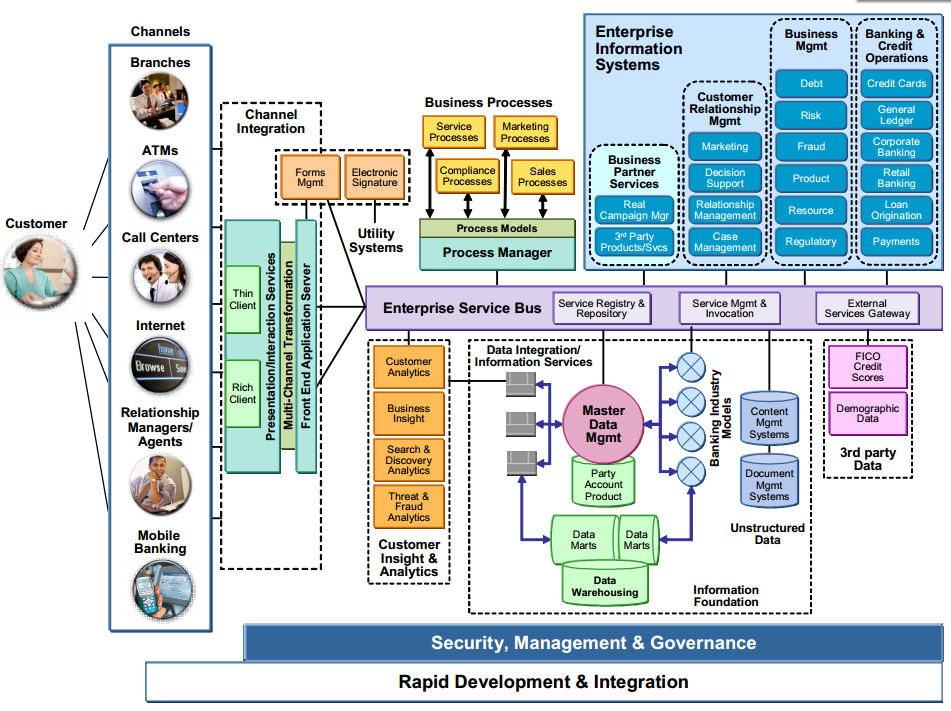
\includegraphics[width=15cm]{img/soa_arch.png}
\caption[Przykładowa architektura SOA.]{Przykładowa architektura SOA. \cite{AnRTeqq}}\label{soa_arch}
\end{centering}
\end{figure}
Rys. [PRZArchSOA] Przykładowa budowa systemu SOA.
Komponenty te można traktować jako tzw. „czarne skrzynki”. Klient korzystający z usługi otrzymuje jedynie interfejs. Implementacja udostępnionych metod nie jest dla niego istotna.
Rozwiązania stosowane w SOA pomagają zapanować nad złożonością systemu. Podstawowa budowa SOA opiera się z reguły na szynie ESB (ang. Enterprsie Service Bus) integrującej poszczególne usługi. ESB jest efektywnym środkiem komunikacji w SOA. Pomaga uwolnić się od sieci powiązań „każdy z każdym”. [SOAidntech] Odpowiada za przesyłanie komunikatów do odpowiednich komponentów. Rozbudowa systemu polega na dołączaniu nowych usług do szyny integracyjnej. 
	
Komunikaty zanim zostaną wysłane do punktu docelowego często poddawane są transformacjom i odpowiedniemu dostosowaniu za pomocą mediacji (ang. mediations) na ESB. Przetworzony komunikat odpowiada formie jakiej oczekuje dostawca usługi.
	
Rejestr SOA (ang. SOA registry) stanowi centralny punkt informacyjny na temat sposobu dostępu, definicji, reguł, bezpieczeństwa i innych danych wymaganych do wykorzystania usług udostępnionych w danym środowisku SOA. Zawiera informacje gdzie poszczególne komponenty SOA są umieszczone. Na jego podstawie ESB potrafi prawidłowo przekierowywać żądanie usługi i ewentualną odpowiedź, a aplikacje i usługi korzystające z usług składowych potrafią skonstruować jej prawidłowe wywołanie. [SOAidntech, SOAfddum]
	
Istotnym elementem w systemach typu SOA jest repozytorium (ang. SOA repository). Stanowi on centralny „magazyn” dla elementów składowych usług takich jak: kod źródłowy, zestawy instalacyjne, specyfikacja itp. Repozytorium usług jest tworzone i wykorzystywane głównie na etapie projektowania usług. [SOAidntech]

\subsection{Usługa sieciowa w SOA}
Usługa sieciowa w SOA (ang. \textit{Web Service}) stanowi usługę świadczoną przez sieć – na przykład Internet. Składnik oprogramowania niezależny od platformy sprzętowej oraz implementacji. Może być zdefiniowany za pomocą języka opisu usług – na przykład bazującym na XML WSDL (ang. Web Service Definition Language), publikowana i wyszukiwana w rejestrze (np. UDDI) oraz wywoływana zdalnie przez opisujący ją interfejs. 
Z reguły Web Service opiera się na konstrukcji uwzględniającej trzy typy komponentów (rys. [WSArchFunc]) : klienta usługi (ang. service requestor), dostawcę usługi (ang. service provider) oraz rejestr usług (service registry) lub broker usług (ang. service broker).  Transport danych w przypadku Web Service z reguły opiera się na HTTP lub HTTPS z wykorzystaniem SOAP. [IBMWebServiceInfo]
Każdy z komponentów jest odpowiedzialny za pełnienie swojej roli:
\begin{itemize}
\item{dostawca usługi tworzy i wdraża Web Service. Publikuje również dostępność opisanego za pomocą WSDL Web Service’u w rejestrze usług (lub brokerze usług),}
\item{rejestr usług lub broker usług odpowiada za rejestrację i kategoryzację opublikowanych usłgu. Dostarcza również możliwość ich wyszukiwania,} 
\item{klienci usług używają rejestru usług (lub brokera usług) do wykrycia Web Service’u opisanego za pomocą WSDL, a następnie wykonują zapytanie do dostawcy usługi. Dostawca usługi udziela odpowiedzi klientowi.}
\end{itemize}

\begin{figure}[h!tbp]
\begin{centering}
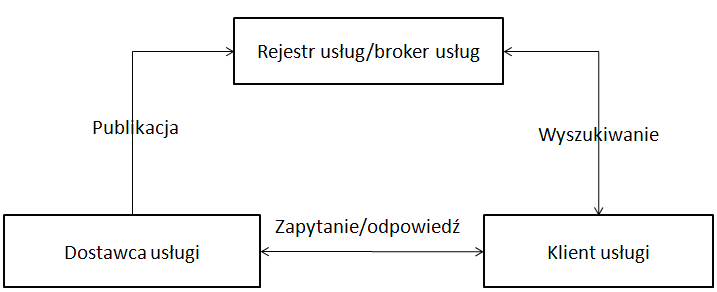
\includegraphics[width=11cm]{img/web_service.png}
\caption[Usługa sieciowa w SOA (Web Service).]{Usługa sieciowa w SOA (Web Service). \cite{AnRTeqq}}\label{soa_arch}
\end{centering}
\end{figure}

\subsection{Warstwy architektury SOA}
W SOA można wyszczególnić dziewięć warstw architektury. Każda z nich składa się z modelu fizycznego oraz logicznego. Model fizyczny opisuje sposób realizacji logiki za pomocą dostępnych technologii oraz produktów, natomiast logiczny zawiera wszystkie architektoniczne bloki, warunki logiczne, decyzje oraz inne - stanowi model konceptualny z dobranym poziomem abstrakcji.

Poszczególne warstwy w SOA to:
\begin{itemize}
\item{Warstwa aplikacji - w jej skład wchodzą wszystkie aplikacje działające w środowisku IT i mające na celu wspieranie działania przedsiębiorstwa. Do przykładów można zaliczyć: aplikacje Java Enterprise lub .NET, systemy transakcyjne, bazy danych oraz systemy ERP i CRM.}
\item{Warstwa komponentów - obejmuje składniki oprogramowania realizujące konkretne operacje usług Odpowiada za fizyczną implementację usługi oraz jej opis dostarczając elementy zgodne z SCA (ang. \textit{Service Component Architecture}) oraz specyfikacją SDO (ang. \textit{Service Data Objects}).}
\item{Warstwa usług - stanowi zbiór wszystkich usług zdefiniowanych za pomocą kontraktu pomiędzy dostawcą, a odbiorcą o sposobie dostarczenia usługi.}
\item{Warstwa procesów biznesowych - w tej fazie tworzona jest kompozycja wielu usług realizujących konkretne biznesowe przypadku użycia. Proces biznesowy składa się z przepływów realizujących dany cel biznesowy organizacji i zagregowanych usług.}
\item{Warstwa prezentacji - stanowi często wspólny interfejs dostępu do usług. Odpowiada za dostarczanie funkcji biznesowych dla klientów końcowych.}
\item{Warstwa integracji - kluczowy element architektury SOA. Jej podstawową funkcją jest zlecenie klientom usług i dostarczanie ich przez dostawców. Przepływ operacji jaki jest wykonywany w tej warstwie to: odbiór zlecenia od klienta, dostarczenie go do dystrybutora, a następnie dostarczenie do klienta.}
\item{Warstwa jakościowa - obejmuje monitorowanie procesów biznesowych odnoszących się do podstawowych wskaźników wydajności danej organizacji. Pełni obserwację pozostałych warstw i informuje o zdarzeniach niezgodnych z zakładanymi.}
\item{Warstwa Business Intelligence - stanowi podstawę do budowania rozwiązań Business Intelligence umożliwiających modelowanie danych analitycznych i eksploracje. W tej warstwie włączane są kluczowe zagadnienia związane z obiegiem informacji w przedsiębiorstwach.}
\item{Warstwa zarządzania - odnosi się do zarządzania wszystkimi elementami cyklu życiu SOA oraz wszystkich warstw architektury (ze szczególnym naciskiem na warstwę jakościową). Wykorzystuje kluczowe wskaźniki wydajności lub efektywności (KPI) do egzekwowania wymagań jakościowych i funkcjonalnych wyspecyfikowanych przez przedsiębiorstwo.}
\end{itemize}
\cite{PlatIntGor}

\subsection{Podstawowe zasady SOA}
Systemy SOA mogą być bardzo różnorodne. SOA nie narzuca konkretnych technologii, a jej realizacja może odbywać się na wiele sposobów. Komunikacja mędzy komponentami w SOA może wykorzystywać różne kanały komunikacji: WS, HTTP, HTTPS, LDAP, FTP, IMAP, JMS, RMI. Budowa systemu SOA może wykorzystywać szynę integracyjną ESB lub broker (można również łączyć wiele szyn ESB ze sobą lub łączyć broker’y z ESB). Mimo tej dużej dowolności istnieje zestaw zasad, na których powinien opierać się każdy system SOA.
\begin{itemize}
\item{luźne powiązania - powiązania odnoszą się do połączeń lub relacji między poszczególnymi elementami. [SOAterlprD] Termin „luźne powiązania” (ang. Loose Coupling) stanowi jeden z fundamentów SOA. [SOAsdj102009] Odwołuje się do sposobu w jaki komponenty SOA współpracują ze sobą.  Zasada „luźnych powiązań” promuje niezależną konstrukcję i ewolucję usług. Każdy z komponentów może pracować autonomicznie wykonując określone czynności. Pracując razem, wymieniają między sobą komunikaty i mogą realizować to co jest zwykle możliwe przez duże, monolityczne aplikacje. „Luźne powiązania” pozwalają również na łatwą dekompozycję komponentów i wykorzystywanie ich do innych celów. [SOAterlprD, SOAidntech]}
\item{interoperacyjność - interoperacyjność (ang. interoperability) opiera się na współpracy pomiędzy systemami. Zapewnienie interoperacyjności jest kolejną bardzo istotną zasadą, o której należy pamiętać tworząc systemy SOA. W miarę rozwoju poszczególnych systemów (np. poprzez dodawanie nowych komponentów) problem integracji staje się coraz trudniejszy do rozwiązania. Należy już na etapie projektowania ograniczać do minimum oraz wybierać odpowiednie protokoły, które dany system będzie obsługiwał. [SOAsdj102009]}
\item{composability - zasada composability jest związana z zachowaniem odpowiednich relacji między komponentami. Systemy, które podążają za ta zasadą cechują się możliwością łączenia swoich komponentów w różne kombinacje w celu spełnienia postawionych wymagań. Umiejętność efektywnego komponowania usług z już istniejących jest kluczowym wymogiem dla osiągnięcia niektórych z najbardziej podstawowych celów przy tworzeniu systemów opierających się na architekturze zorientowanej na usługi. [SOAterlprD]}
\item{reużywalność - każda tworzona usługa powinna zachowywać zasadę reużywalności (ang. reusability).  Opiera się ona na takim projektowaniu usług, aby była możliwość wielokrotnego jej wykorzystania do tworzenia kolejnych usług. [SOAsdj102009]}
\item{kontraktowość usług - każda usługa powinna mieć zdefiniowany kontrakt (ang. service contract), który zawierany jest każdorazowo pomiędzy usługą, a jej konsumentem. Wyrażane są przez nie cele i możliwości danej uslugi. [SOAterlprD] W kontraktach znajdują się również opisy informacji oferowanych  i oczekiwanych przez usługi. [SOAinfoq10]}
\item{abstrakcyjność - zasada abstrakcji (ang. abstraction) zakłada, że kontrakty usług mogą zawierać jedynie niezbędne informacje i mogą udostępniać jedynie te informacje, które są w nich zdefiniowane. Zasada ta podkreśla potrzebę ukrycia przez usługi tak wielu informacji jak to tylo możliwe. [SOAterlprD]}
\item{autonomiczność usług - autonomia usługi (ang. service autonomy) jest kolejnym paradygmatem projektowania systemów typu SOA. Termin ten odwołuje się do usług o podwyższonej niezależności od środowisk wykonawczych. [SOAsrvautoWCSS] Usługa powinna mieć możliwość podmiany środowiska wykonawczego z lekkiego prototypowego (ang. lightweight prototype) do pełnowymiarowego (ang. full-blown), w którym są już uruchomione inne usługi odwołujące do niej. Zgodnie z zasadą autonomii każda z usług może być wdrażana, wersjonowana i zarządzana niezależnie od innych. [SOAinfoq10]}
\item{wykrywalność usług - zasada wykrywalności usług (ang. services discoverability) polega na tym, że usługi powinny być opisywane za pomocą meta danych w takich sposób, aby były efektywnie wyszukiwane, przetwarzane i interpretowane zarówno w czasie projektowania jak i wykonywania. [SOAinfoq10, SOAsrvautoWCSS]}
\item{spójność i ziarnistość usług - interfejsy usług w systemach SOA powinny być tak zaprojektowane, aby wiązały tylko określony zbiór wymagań biznesowych. \cite{SOAsdj102009} Należy zadbać o optymalną ziarnistość interfejsów dla obsługiwanych typów i rozmiarów danych (ziarnistość danych wejściowych i wyjściowych), wartości biznesowej oraz funkcjonalności (domyślna i parametryzowana ziarnistość funkcjnonalności). [SOAdefgranaaImp]}
\item{bezstanowość usług - zasada bezstanowości usług (ang. Services statelessness) odwołuje się do minimalizacji użycia zasobów i ograniczania się do przechowywania i przetwarzania tylko absolutnie niezbędnych informacji.  [SOAsrvautoWCSS ] Usługa nie może być w stanie przetrzymywać informacji o wcześniejszych żądaniach klienta. Każda z informacji powinna być odizolowana od innych. Skuteczne stosowanie zasady bezstanowości może znacząco zwiększyć wydajność rozwiązania oraz zmniejszyć współbieżne działanie usług. \cite{SOAsdj102009}}
\item{enkapsulacja - enkapsulacja (ang. Encapsulation) stanowi jedną z podstawowych zasad poprawnego projektowania systemów typu SOA. Zapewnienie odpowiedniej hermetyzacji dla usług sprowadza się do ukrywania szczegółów konfiguracyjnych oraz implementacyjnych danej usługi.}
\end{itemize}

\subsection{Korporacyjna szyna usług - ESB}
ESB (ang. \textit{Enterprise Service Bus}) stanowi abstrakcyjną warstwę wymiany komunikatów. W systemie informatycznym wprowadza znaczną elastyczność, ponieważ pozwala na dynamiczne przyłączanie i odłączanie usług.\cite{PlatIntGor}

Głównym celem korporacyjnej szyny usług jest dostarczanie pewnego rodzaju wirtualizacji dla korporacyjnych zasobów pozwalając na rozwijanie logiki biznesowej niezależnie od infrastruktury lub sieci oraz bez potrzeby pisania dodatkowego kodu. Zasoby w ESB są modelowane jako usługi, które oferują jedną lub więcej operacji biznesowych.\cite{IBMRBSoaPat}

Dobra praktyka projektowania architektury systemu zapewnia, że wszystkie połączenia między aplikacjami będą realizowane z wykorzystaniem szyny.\cite{PlatIntGor} Pełne sprostanie różnorodności wzorców integracji jakie oferuje SOA wymaga utrzymywania przez ESB trzech głównych paradygmatów integracji aplikacji korporacyjnych:
\begin{itemize}
\item{Architektura zorientowana na usługi - rozproszone aplikacje zbudowane są z ziarnistych usług wieleokrotnego użytku z dobrze zdefiniowanymi, opublikowanymi i zgodnymi ze standardami interfejsami.}
\item{Architektura zorientowana na komunikaty (ang. \textit{message-driven architecture}) - aplikacje wysyłają komunikaty między sobą.}
\item{Architektura zorientowana na zdarzenia (ang. \textit{event-driven architecture}) - aplikacje generują i konsumują usługi niezależnie od pozostałych.} \cite{IBMRBSoaPat}
\end{itemize}

Stosowanie szyny integracyjnej wiąże się z wieloma zaletami. Przede wszystkim powoduje zmniejszenie kosztów dzięki szybkiemu i elastycznemu rozwiązaniu integracji eliminującym połączenia typu \textit{point-to-point}. ESB umożliwia również rozwój obecnych środowisk bez wpływu na obecne co pozwala na łatwe rozszerzanie systemu o nowe funkcjonalności.\cite{IBMRBSoaPat}

\section{Adaptacja SOA w architekturze korporacyjnej}
Tworzona architektura koroporacyjna powinna dążyć do możliwe jak największego zapewnienia interoperacyjności tworzonych rozwiązań informatycznych i łatwą ich integrację. 

\chapter{Metodyki projektowania rozwiązań w architekturze usługowej}

\section{Wstęp}


\section{RUP4SOA}
\subsection{Czym jest RUP?}
RUP (ang. \textit{Rational Unified Process}) stanowi proces  wytwarzania oprogramowania oparty na iteracjach. Metodyka ta została zdefiniowana przez grupę Rational Software (przejętą przez firmę IBM w roku 2003). 

RUP zapewnia zdyscyplinowane podejście do przydzielania zadań i obowiązków w ramach rozwoju organizacji. Celem podstawowym tej metodyki jest dostarczenie wysokiej jakości oprogramowania spełniającego potrzeby użytkowników końcowych w zgodzie z harmonogramem i ramami budżetowymi.
\cite{RUPIntRat} Stanowi przede wszystkim bardzo duży zbiór praktyk, który może być dostosowywany i rozszerzany w celu jak najlepszego dopasowania się do danej organizacji. Charaktertystyczne dla metody jest rozwój sterowany przypadkami użycia (ang. \textit{Use Case Driven Development}).\cite{RUPMartFow}

W RUP można wyróżnić poszczególne fazy:
\begin{itemize}
\item{faza początkowa (ang. \textit{inception}) – wstępne określenie wymagań, ryzyka, kosztu, harmonogramu, a także architektury systemu,}
\item{faza opracowania (ang. \textit{elaboration}) – ustalenie wymagań (większości przypadków użycia), architektury systemu oraz planu całego procesu wytwarzania systemu,}
\item{faza konstrukcji (ang. \textit{construction}) – tworzenie systemu (kolejnych komponentów), w trakcie następuje oddanie pierwszej (i być może dalszych) wersji użytkownikowi,}
\item{faza przekazania (ang. \textit{transiation}) – system jest przekazywany użytkownikowi, wdrażany, szkoleni są pracownicy obsługi systemu, następuje walidacja i końcowe sprawdzenie jakości.}\cite{RUPIntRat}
\end{itemize}
\subsection{Wykorzystanie RUP w projektowaniu SOA}
RUP4SOA stanowi modyfikację metodyki RUP i dołączono do niej zadania i produkty potrzebne przy projektowaniu rozwiązań w architekturze usługowej. RUP4SOA stanowi komercyjny plug-in dla framework'a RUP. Rozszerza standardowy pakiet o zbiór dodatkowych artefaktów i właściwości. W odróżnieniu od klasycznego RUP, metodyka ta opiera się na wyróżnieniu trzech dyscyplin związanych z analizą i projektowaniem:
\begin{itemize}
\item{analiza i projektowanie architektury SOA - przygotowanie architektury SOA zgodnie z wymaganiami,}
\item{analiza i projektowanie kontraktów w architekturze SOA - analizie poddane są procesy integracyjne, związane z dostarczaniem usług i realizacją kontraktów między organizacjami,}
\item{analiza i projektowanie logiki usług SOA - identyfikacja usług w systemach informatycznych w jednostkach, w których wdrażana będzie architektura SOA}
\end{itemize}
Reszta dyscyplin jest analogiczna do metodyki RUP. \cite{PlatIntGor} W RUP4SOA można wyróżnić poszczególne fazy:
\begin{itemize}
\item {modelowanie biznesowe,}
\item {specyfikacja wymagań,}
\item {analiza i projektowanie architektury SOA,}
\item {analiza i projektowanie kontraktow SOA,}
\item {analiza i projektowanie logiki usług,}
\item {implementacja,}
\item {testowanie,}
\item {wdrożenie,}
\item {zarządzanie zmianą i konfiguracją,}
\item {zarządzanie projektem,}
\item {środowisko.}
\end{itemize}

W fazie analizy i projektowania przygotowywana jest architektura SOA zgodnie z postawionymi wymaganiami i modelem biznesowym. Istotne jest, aby opracowywana architektura była projektowana z zamysłem o jak najprostszej realizacji i późniejszym wdrożeniu. Kolejną dyscyplinę stanowi analiza i projektowanie kontraktów w architekturze usługowej. Ta faza opiera się na analizie procesów integracyjnych związanych z dostarczaniem usług i wymianą kontraktów między organizacjami. Następny element metodyki RUP4SOA stanowi analiza i projektowanie logiki usług SOA, który powiązany jest z identyfikacją usług informatycznych w organizacjach. 

Po fazach analizy i projektowania następują kolejno implementacja oraz testy. W następnym etapie utworzony produkt zostaje wdrożony na przygotowane środowisko. Równolegle trwają również prace związane z zarządzaniem projektem, konfiguracją oraz zmianami. \cite{PlatIntGor}

Podstwowym produktem wytworzonym przez Architekta oprogramowania w przypadku RUP4SOA jest model usług. Do podstawowych zadań Architekta oprogramowania zalicza się realizację fazy "identyfikacji usług".

Projektant w RUP4SOA odpowiada za przygotowanie projektu usługi, a jego odpowiedzialność jest związana z produktami: komunikat, usługa, kanał usługi, bramka usługi, współpraca usługi, partycja usługi, specyfikacja usługi oraz komponent usługi. 

\subsection{Zalety i wady RUP4SOA}
RUP4SOA jest jedną z najpopularniejszych metodyk stosowanych do projektowania architektury usługowej. Największy nacisk kładzie na fazy związane z analizą i projektowaniem systemu informatycznego - rozszerzonym o elementy związane z usługami sieciowymi. Fakt ten może powodować większą zgodność między wyobrażnieniami klienta, a rzeczywistym produktem w formie systemu. 

Jedną z jej największych zalet jest również opieranie się na metodyce RUP, która wykorzystuje doświadczenia i praktyki przyjęte przez organizacje na przestrzeni wielu lat. \cite{JonSimRUPSoa}

Metodyka ta nie specyfikuje wielu elementów istotnych do budowy rozwiązań integracyjnych. Skupia się na projektowaniu pojedynczego systemu, który może być jedynie włączony do platformy integracyjnej. \cite{PlatIntGor}

\section{SOMA}
\subsection{Czym jest SOMA?}
SOMA (ang. \textit{Servie-Oriented Modeling and Architecture} stanowi kolejną metodykę projektowania systemów w architekturze usługowej. \cite{PlatIntGor} Metoda cyklu rozwoju oprogramowania definiująca kluczowe techniki i opisująca poszczególne role w projekcie SOA oraz struktury podziału pracy (WBS - ang. \textit{Work Breakdown Structure}). WBS obejmuje zadania związane z wejściowymi i wyjściowymi produktami pracy, z normatywnymi wskazówkami do szczegółowej analizy, projektowaniem, implementacją i wdrażaniem usług oraz komponentów potrzebnych do budowy wydajnego, reużywalnego środowiska.

SOMA została utworzona i jest rozwijana przez firmę IBM. W swoim podejściu metodyka wykorzystuje wiele elementów z Worldwide Project Management Method (jedna z metodyk zarządzania projektami). \cite{SOMAArsIBMJour}

\subsection{Fazy metodyki SOMA}
SOMA bazuje na siedmiu podstawowych fazach:
\begin{itemize}
\item{modelowanie biznesowe (ang. \textit{business modeling and transformation}),}
\item{zarządzanie rozwiązaniem (ang. \textit{solution management}),}
\item{identyfikacja (ang. \textit{identification}),}
\item{specyfikacja (ang. \textit{specification}),}
\item{realizacja (ang. \textit{realization}),}
\item{implementacja (ang. \textit{implementation}),}
\item{monitorowanie i zarządzanie (ang. \textit{monitoring and management}).}
\end{itemize}

Poszczególne fazy nie następują po sobie w sposób liniowy. SOMA opiera się na iteracyjnym, przyrostowym podejściu do realizacji rozwiązań SOA. Powoduje to łagodzenie ryzyk projektowych oraz wynika z cyklu życia usług w modelu SOA. Zadania związane z budową rozwiązań informatycznych realizowane są w niej w podobny sposób bez względu na zakres. 

Można również mówić o fraktalnej charakterystyce metodyki. Każda kolejna  iteracja (ang. \textit{successive iteration} jest powiązana z pojęciem ewolucji usług. Opiera się nie tylko na ryzykach dotyczących implementacji, ale również na zależnościach związanych ze zbiorem usług, gdy usługi zmieniają się w trakcie cyklu życia systemu. W SOMA przypisywanie priorytetów w Modelu usług odbywa się z wykorzystaniem diagramów zależności usług (ang. \textit{service-dependency diagram}. Na podstawie ryzyk związanych z architekturą rozwiązania wyłaniany jest podzbiór usług przewidywany do implementacji w kolejnej iteracji.

\begin{figure}[h!tbp]
\begin{centering}
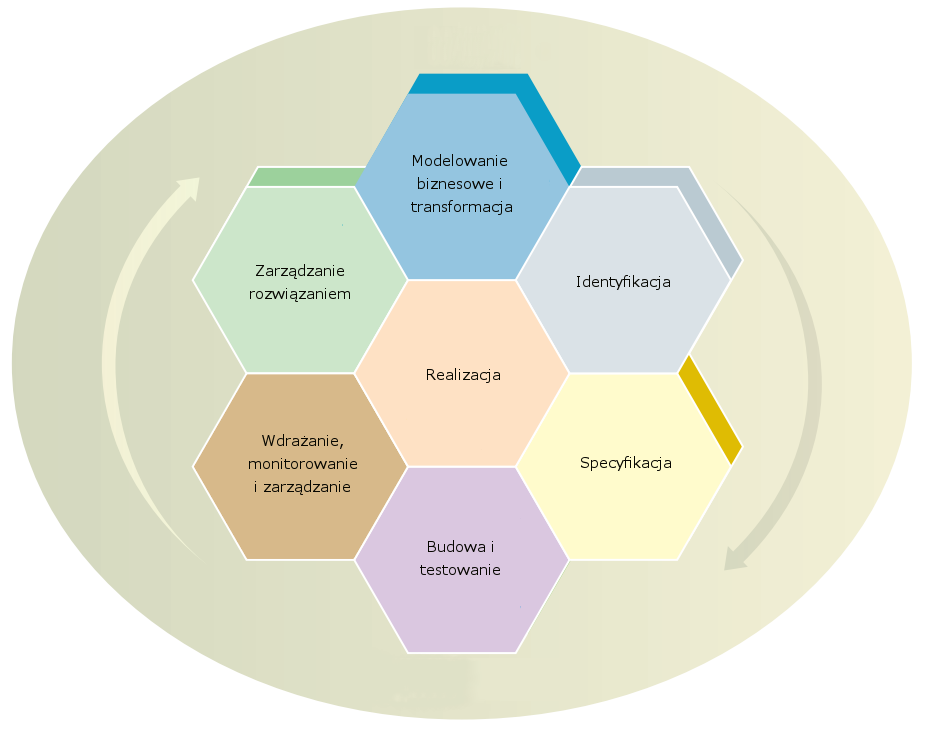
\includegraphics[width=14cm]{img/soma_fractal_lifecycle.png}
\caption[Fraktalne podejście do budowy systemów - fazy metodyki SOMA.]{Fraktalne podejście do budowy systemów - fazy metodyki SOMA. \cite{SOMAArsIBMJour}}\label{soma_fractal_lifecycle}
\end{centering}
\end{figure}

Charakterystyczną cechą dla SOMA jest również pojęcie przypadku usługowego (ang. \textit{service case}), który identyfikuje "reużywalny" (ang. \textit{reuse}) zbiór operacji usługi. Ważne jest, aby zidentyfikować taki zestaw usług, który łącznie pozwala na spełnienie celów biznesowych. \cite{PlatIntGor}

W fazie modelowania biznesowego i transformacji funkcjonowanie organizacji jest modelowane, symulowane i optymalizowane. Na tym etapie wyszczególnia się również główny obszar przekształcenia danej jednostki - podstawowy dla kolejnych projektów opierających się na pozostałych fazach SOMA. Modelowanie biznesowe i transformacja jest opcjonalnym elementem metodyki, ale ściśle zalecanym. 

Realizacje SOA mają hybrydową naturę i z reguły obejmują wiele typów rozwiązań. W fazie zarządzania rozwiązaniem inicjowany jest projekt oraz wybierany odpowiedni scenariusz realizacji. Występuję kilka możliwych scenariuszy: wytwarzania oprogramowania (ang. \textit{custom development}), integracji pakietów aplikacji (ang. \textit{package application integration}). W tym etapie tworzona jest również konfiguracja metodyki dostosowana do potrzeb danego projektu. Ponadto zdefiniowaniu podlegają: zadania, role, produkty pracy oraz poradniki.\cite{SOMAArsIBMJour}

Faza identyfikacji związana jest z identyfikacją trzech elementarnych dla SOA konstrukcji: usług, komponentów oraz usług.\cite{PlatIntGor} Do zadań tego etapu należy: dekompozycja obszarów biznesowych (Domain Decomposition), modelowanie usług w kontekście celów biznesowych (Goal-Service Modeling) oraz analiza istniejących zasobów IT (Existing Assets Analysis).\cite{SOMAibmRosSuda} Do produktów końcowych tej fazy zalicza się listę kandydujących usług do realizacji oraz powiązań między nimi. \cite{PlatIntGor}

Podczas specyfikacji usług projektowane jest rozwiązanie. Powstaje projekt podstawowy oraz niektóre elementy projektu szczegółowego. Analizowane są zasoby IT pod kątem zależności ze zidentyfikowanymi usługami w poprzedniej fazie, przepływami oraz zdarzeniami. Metodologia dostarcza gotowe szablony, wzorce oraz techniki wykorzystywane w celu określenia usług, przepływów i komponentów. 

W skład fazy specyfikacji wchodzą następujące elementy:
\begin{itemize}
\item{Identyfikacja zależności między usługami - w oparciu o szczegółowy przegląd danej usługi możliwe jest odkrycie jej zależności z innymi usługami lub aplikacjami. Mogą okazać się one niezbędne do dostarczenia niektórych funkcjonalności.}
\item{Test papierka lakmusowego (ang. \textit{service litmus test} - powiązany z podejmowaniem decyzji dotyczących ekspozycji.}
\item{Identyfikacja kompozycji usług i przepływów - przegląd procesów biznesowych oraz obszarów funkcjonalnych umożliwia ustalenie kompozycji usług z innych usług i ich przepływów dostarczających pożądaną funkcjonalność biznesową.}
\item{Identyfikacja wymagań niefukncjonalnych - wymagania definiujące oczekiwany poziom usług.}
\item{Definicja specyfikacji komunikatów - obejmuje identyfikację i specyfikację formatu oraz zawartości komunikatów wejściowych i wyjściowych dla usług.}
\item{Dokumentacja decyzji dotyczących zarządzania stanem.}
\end{itemize}

Faza realizacji związana jest ze sprawdzaniem stabilności i realizowalności zaprojektowanego rozwiązania poprzez budowę prototypów. Zadanie to powinno mieć miejsce we wczesnym etapie projektu, aby zminimalizować niepowiedzenia i wyeliminować niepotrzebne ryzyka. Faza ta stanowi pewnego rodzaju formę technicznego studium wykonywalności. Każdy poziom rozwiązania wiąże się również z wybieranym podejściem lub sposobem realizacji prac.

W skład fazy realizacji wchodzą następujące czynności:
\begin{itemize}
\item{iteracyjna alokacja usług do komponentów,}
\item{przypisanie komponentów w warstwach znajdujących się w architekturze aplikacji,}
\item{identyfikacja i oszacowanie ograniczeń technologicznych, które mogą wpływać na realizowalność zadań.}
\end{itemize}

W fazach implementacji i wdrożenia oraz monitorowania i zarządzania są konstruowane, generowane i łączone usługi, komponenty funkcjonalne i techniczne oraz przepływy. Konstruowane są również poszczególne elementy opakowujące oraz odpowiednie mechanizmy dla istniejących komponentów. Wykonywane są również testy: integracyjne, jednostkowe, komponentów, przepływów oraz systemu dla usług. \cite{PlatIntGor, SOMAArsIBMJour}

\subsection{Produkty SOMA}
Stosowanie SOMA przynosi rezultaty między innymi w postaci utworzonych modelów - usług i informacji. 

Model usług zawiera zbiór informacji dotyczących aktualnie zidentyfikowanych usług w organizacji, które będą wykorzystane do realizacji założonych celów biznesowych oraz procesów. W modelu tym znajdują się również dane opisujące kwestie: biznesowe, funkcjonalne, niefunkcjonalne oraz dotyczące technicznej realizacji. Wyszczególnione są również informacje o hierarchii złożoności, ekspozycji, zależności między usługami oraz wymagania związane z poziomem jakości. 

Model informacji odpowiada za kontekst biznesowy. Zawiera elementy takie jak: model koncepcyjny, decyzje dotyczące realizacji oraz relacje i ekspozycję encji.

Oprócz wymienionych modeli metodyka SOMA dostarcza również elementy: kontekst biznesowy, definicję procesów, identyfikację procesów, katalog reguł biznesowych oraz listę zdarzeń biznesowych.

\subsection{Zalety i wady SOMA}
Stosowanie metodyki SOMA może przynosić szereg korzyści. 

Model usług stanowiący końcowy rezultat etapu modelowania pozwala na łatwe i szybkie opracowanie projektu technicznego, implementację nowych usług oraz udostępnienie usług na podstawie już istniejących. 

Ponadto SOMA pozwala zdefiniowanie i zaprojektowanie poszczególnych serwisów technicznych na poziomie biznesowym, tak aby zwiększyć elastyczność organizacji do zmiennych biznesowych oraz zredukować koszty wdrażania nowych usług.

//TODO: DODAĆ WADY

\chapter{Przegląd języków do projektowania systemów informatycznych o architekturze SOA}
\section{SoaML}

\subsection{Czym jest SoaML?}


\subsection{Główne elementy notacji}
\subsection{Modelowanie z wykorzystaniem SoaML}
\section{ArchiMate}
\section{Inne języki}

\chapter{Opracowanie metody projektowania systemów informatycznych o architekturze SOA}
Kontrola złożoności systemu.

\chapter{Weryfikacja koncepcji na przykładzie systemu bankowego}
\section{Projektowanie systemu bankowego w oparciu o utworzoną koncepcję}
\subsection{Opis ogólny}
\subsection{Analiza systemu}
\subsection{Implementacja}
\subsection{Proces wdrożenia}
\subsection{Testy}
\section{Cel systemu w odniesieniu do zaprojektowanej koncepcji}
\chapter{Podsumowanie i wnioski}
